\documentclass[a4paper, 12pt]{article}
\usepackage[ngerman]{babel}
\usepackage{amsmath}
\usepackage{amsfonts}
\usepackage{listings}
\usepackage{pgfplots}
\usepackage{graphicx}
\pgfplotsset{compat=1.9}
\usepackage{tikz}
\usepackage{float}
\author{Lukas Hofmaier}
\title{Userbased Collaborative Filtering und Matrixfaktorisierung}
\begin{document}

\lstset{basicstyle=\small,
language=Haskell,
stringstyle=ttfamiliy
}

\maketitle
\newpage
\tableofcontents
\newpage
\begin{abstract}
  Recommender Systeme nutzen Datenbanken mit Userpreferenzen, um dem User aus einer grossen Menge von Objekten, diejenigen zu empfehlen, die er noch nicht gesehen hat. Dieser Report konzentriert sich auf Collaborativ Filtering. Collaborative Filtering ist eine Klasse von Recommender, die Empfehlungen aufgrund von Preferenzen anderer User berechnet.
In diesem Report werden zwei Collaborative Filtering Methoden beschrieben. Userbase Collaborative Filtering ist eine der ersten und intuitivsten Methoden. Matrixfaktorisierung ist eine weitere Methode, die an der Netflix Competition die besten Resultate lieferte.

Die Algorithmen werden mit einer geeigneten Evaluation verglichen. Die Evaluation und die Algorithmen wurden in Haskell implementiert.

\end{abstract}

\section{Recommender-Problem}
\label{sec:problem}
Dieser Abschnitt beschreibt was ein Recommendersystem ist und weshalb es einen Mehrwert schaffen kann.

Konsumenten werden heute in vielen Bereichen mit einer un"uberschaubaren Anzahl an Kaufm"oglichkeiten konfrontiert. In einem Webshop f"ur B"ucher oder Filme ist es es f"ur den Konsumenten beispielsweise schwierig, alle Artikel im Angebot anzuschauen und aufgrund dieser Evaluation die besten Artikel auszuw"ahlen. Beim Recommender-Problem geht es darum aus einer Mengen von Artikel (Items) ein sortierte Liste mit den empfehlenswertesten Artikel f"ur einen spezifischen Kunden (User) zu erstellen. Recommender kommen vorallem dort zum Einsatz, wo pers"onlicher Geschmack bei der Bewertung von Artikel eine wichtige Rolle spielt.

Ein Recommendersystem kann eine Bewertung absch"atzen (vorhersagen), die ein bestimmter User einem bestimmten Item gibt. Recommender berechnen die Bewertungen f"ur Items, die der User noch nicht gesehen hat. Die Items mit den besten Bewertungen werden dem User empfohlen.

Recommendersysteme werden vorallem im e-Commerce eingesetzt. Man kann sie aber auch dazu verwenden um unwichtige Informationen von wichtigen zu trennen. Recommender k"onnen beispielsweise auch f"ur Information Retrieval eingesetzt werden. Sie generieren eine Liste von Dokumenten die der User noch nicht gesehen hat \cite{herlocker00}.

In nachfolgenden Text wird haupts"achlich von User und Items gesprochen. Sie sind folgendermassen definiert.

\begin{description}
\item[User] User sind die Konsumenten oder f"ur die eine Empfehlung erstellt werden soll. 
User haben Preferencen und bewerten Items aufgrund des pers"onlichen Geschmacks. In einer Information Retrieval Anwendung k"onnen User auch einfach die Benutzer der Software sein.
\item[Item] 
Items k"onnen Artikel, Filme, B"ucher, Dokumente e.t.c sein. Items werden den Usern empfohlen.
\end{description}

Der aktive User bezeichnet den User, f"ur den Empfehlungen erstellt werden soll \cite{jannach11}.

Es gibt zwei unterschiedliche Strategien f"ur Recommendersysteme: Content filtering und Collaborative Filtering. Dieser Report besch"aftigt sich nur mit Collaborative Filtering Methoden. 

\subsection{Content based Filtering}
\label{sec:contentbased}

Bei Content-based Filtering wird zu jedem Artikel und zu jedem User ein Profil erstellt. Dieses Profile enth"alt Informationen "uber die Eigenschaften von User und Item. Beispielsweise k"onnte man alle angebotenen Filme nach ihrer Genrezugeh"origkeit bewerten. Ein Film hat beispielsweise einen Action und einen Romantikanteil. User k"onnen angeben, ob sie lieber Action oder Romantik m"ogen. Content based Filtering sucht dann Filme, die am besten mit dem Userprofile matchen. Die Schwierigkeit an Content based Filtering ist das Erfassen von Daten zu jedem Item und zu jedem User. Jemand muss jeden Artikel im Angebot nach seinem Content bewerten. Von jedem User muss ein Profil erstellt werden. Der User kann seine Preferenzen oft selber eingeben. Denn meisten User ist das zu m"uhsam.

\subsection{Collaborative Filtering}
\label{sec:collaborativefiltering}

Collaborative Filtering ist eine weitere M"oglichkeit das Re\-commender-Prob\-lem zu l"osen. Bei Collaborative Filtering wird das Verhalten von User in der Vergangenheit analisiert. Dabei werden Bewertungen oder Transaktionen angeschaut. Der Inhalt der Artikel ist egal. Da diese Strategie unab"angig vom Inhalt ist kann sie f"ur jedes beliebige Recommendersystem eingesetzt werden. Es kann also im e-Commerce sowie auch im Information Retrieval eingesetzt werden.  Es wird in vielen Webshops erfolgreich eingesetzt \cite{sarwar01}. 

Ziel des Collaborative Filtering ist, es einem User neue Items oder f"ur ein bestimmtes Item und einen bestimmten User eine Bewertung vorauszusagen. Typischweise gibt es eine Menge von $m$ Usern  $\mathnormal{U}$ und eine Menge von $ \mathnormal{I} $ Items. Jeder User $\mathnormal{u}$ hat eine Liste $\mathnormal{I_u}$ von Items, welche er bewertet hat. Diese Bewertung wird meisten als numerischer Wert in einem Intervall ausgedr"uckt. Bei Filmen hat es sich zum beispiel durchgesetzt das man eine Zahl zwischen 1 und 5 angibt, wobei die 5 aussagt, dass der Film dem User gefallen hat und eine 1 bedeutet, dass dem User der Film nicht gefallen hat.. Diese Bewertungen werden von den User explizit eingegeben oder sie werden zum beispiel vom Kaufverhalten abgeleitet.

\subsubsection{Abgrenzung zu Contentbased Filtering}
\label{sec:definitioncf}

Bei Collaborative Filtering geht man davon aus, dass man die Bewertungen anderer User dazu benutzen kann, um dem aktiven User ein Item zu empfehlen, dass er noch nicht gesehen hat. Im Unterschied zu Contentbased Filtering ist der Inhalt des Items f"ur die Empfehlung nicht relevant. Das einzige was z"ahlt sind die Bewertungen anderer User.

\subsubsection{Vor- und Nachteile}
\label{sec:advandage}

Gegen"uber Contentbased Filtering bietet Collaborative Filtering folgenden Vor- und Nachteile.
\begin{description}
\item[Kein Wissen "uber Inhalt n"otig] Es muss nicht jedes Item nach seinem Content dursucht werden. Meisten ist der Inhalt im Kontext der Empfehlung nicht brauchbar (L"ange, Kategorie, Jahr).
\item[Usergeschmack "andert] Collaborativ Filtering passt sich automatisch an.
\item[Intuitiv] Jeder versteht "Kunden die diesen Artikel gekauft haben, haben auch diese Artikel gekauft.
\end{description}

\subsubsection{Resultate von Collaborative Filtering}
\label{sec:output}

Man kann zwei Resultate von Collaborative Filtering unterscheiden (siehe Abbildung \ref{fig:cfprocess}.

\begin{description}
\item[Prediction] Das System berechnet eine wahrscheinliche Vorhersage $P_{u,i}$ f"ur eine Bewertung von Item i und User u
\item[Empfehlung] Das System gibt eine Liste von $N$ Items zur"uck, die Items in der Liste hat der user noch nicht bewertet und das System hat die h"ochsten Bewertungen f"ur den aktiven User berechnet.
\end{description}

\begin{figure}
  \centering
      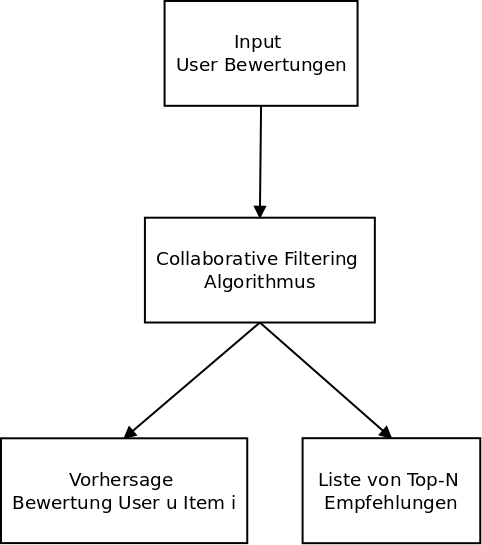
\includegraphics[width=0.5\textwidth]{cf}
  \caption{Collaborative Filtering Prozess}
  \label{fig:cfprocess}
\end{figure}

\subsubsection{Nearest-Neighbor vs. Latent Factor Models}
\label{sec:cfmodels}

Collaborative Filtering kann weiter in zwei unterschiedliche Methoden aufgeteilt werden:

\begin{description}
\item[Neighboorhood Methoden] Bei Neighboorhood Methoden werden f"ur jeden User "ahnliche User gesucht. Es wird eine Nachbarschaft mit "ahnlichen User erstellt.
"Ahnlichkeit wird aufgrund von gemeinsam bewerteten Item berechnet. Wenn zwei User f"ur mehrere Items die selben Bewertungen vergeben, sind sie sich "ahnlich. Sie haben einen "ahnlichke Einem User werden diejenigen Items empfohlen, die er noch nicht kennt und die eine hohe Bewertung von "ahnlichen Usern erhalten haben.
M"ochte man das Rating von einem User f"ur ein bestimmtes Item ab\-sch"atz\-en, schaut man, ob User in der Nachbarschaft das Item bereits bewertet haben. Aufgrund der "Ahnlickeit und den vorhandenen Ratings berechnet man das Rating das der User f"ur dieses Item abgeben w"urde.
\item[Latent Factor Model] Latent Factor Modelle repr"asentieren User und Items als Vektoren. Die Elemente sind Prefenzen und Eigenschaften. Diese Vektoren werden aufgrund der vorhandenen Bewertungen berechnet.
\end{description}

Dieser Report beschreibt Algorithmen f"ur beide Modele. Userbased ist eine Neighborhood Methode. Matrixfaxtorisation nutzt ein Latent Factor Model.

\subsection{Herausforderungen}
\label{sec:challenges}

Bei der Implementierung von Recommendersystemen ergeben sich mehrere Herausforderungen.

\begin{description}
\item[Genauigkeit] Die Differenz der Empfehlungen, die das Recommendersystem macht, soll so wenig wie m"oglich von der tats"achlichen Bewertung abweichen.
\item[Skalierbarkeit] 
Collaborative Filtering muss f"ur Millionen User und Items m"oglich sein. Die Technik soll also f"ur grosse Datenmengen skalieren.
\item[Sparsity] F"ur eine grosse Menge an Items gibt es in der Regel nur eine kleine Anzahl an Items, die ein User auch bewertet hat. Wenn sich keine gemeinsamen Items zwischen den Usern finden k"onnen auch keine Nachbarschaften gebildet werden.
\end{description}

\section{Evaluation}
\label{sec:evaluation}

In diesem Report werden mehrere L"osungen f"ur das Recommenderproblem beschrieben. Um die Qualit"at der Methoden zu messen werden die unterschiedlichen L"osungen miteinander verglichen. Die Qualit"at wird durch die Genauigkeit der Bewertungsvorhersagen beschrieben. Man misst die Differenz zwischen vorhergesagter und tats"achlicher Bewertung.

Dieser Abschnitt beschreibt eine Methode um die Qualit"at der Algorithmen zu evaluieren. In den nachfolgenden Abschnitten werden die Algorithmen mit dieser Methode evaluiert und miteinader verglichen.

\subsection{Daten}
\label{sec:data}

Ein Recommenderalgorithmus ben"otigt Daten um das Model zu erstellen. F"ur die Evaluation sind ebenfalls vorhandende Bewertungen notwendig. Diese Daten liegen oft in Form einer Matrix vor. Die Zeilen rep"asentieren Items und die Kolonnen User. In den Zellen steht welche Bewertung ein User einem Item gegeben hat. Diese Matrix nennt man Ratingmatrix.

Die Daten f"ur Recommender Systeme k"onnen auf zwei unterschiedliche Arten beschafft werden.

\begin{description}
\item[Explizites Feedback] Bei explizitem Feedback verl"asst man sich auf Daten die User explizit eingegen haben. Beispielsweise werden User aufgefordert, dem System ihre Preferenzen anzugeben oder man pr"asentiert den User eine Reihe von Items, die er auf einer Skala von 1 bis 5 bewerten muss. Ein Problem von explizitem Feedback ist, dass es oft zu d"unn besetzten Ratingmatrizen f"uhrt, da die User keine Zeit haben um alle verf"ugbaren Items zu bewerten.
\item[Implizites Feedback] Implizites Feedback leitet die Bewertungen der User f"ur Items aus Beobachtungen ab. Das System beobachtet die Interaktionen, wie zum Beispiel in Vergangheit gekaufte Artikel, Browsehistory, Suchanfragen oder Klickverhalten, des User mit dem System. Oft besteht implizites Feedback nur aus boolschen Werten. Das heisst entweder ein Ereignis ist eingetreten oder nicht.
\end{description}

 Der User-based Collaborative Filtering Algorithmus berechnet zu jedem User-Paar eine "Ahnlichkeit und zu jedem User eine Nachbarschaft. Das System berechnet die "Ahnlichkeiten auftrund der Ratingmatrix. Diese gibt Auskunft dar"uber, welche Bewertung die User den Items gegeben haben.

\subsubsection{MovieLens Daten}
\label{sec:movielens}

F"ur das Projekt wurden die Daten von Movielens verwendet. MovieLens wurde von vom GroupLens Projekt an der Universit"at Minnesota entwickelt. Die Daten werden mit einer Webanwendung gesammelt. User k"onnen Filme bewerten und MovieLens gibt den User darauf eine Top-N Empfehlungsliste. Die Daten k"onnen von http://www.grouplens.org/node/12 heruntergeladen werden. 

Das Datenset enth"alt die Bewertung von 943 User und 1682 Items. Die Daten sind in Kolonnen strukturiert. Die erste und zweite Kolonne enth"alt User und Item ID. Die dritte Kolonne enth"alt ein Zahl zwischen 1 und 5. Die repr"asentiert die Bewertung. Und in der vierten Kolonne ist ein Timestamp der Bewertung. Das Movielens Datenset enth"alt insgesamt 100000 Bewertungen. Abbildlung \ref{fig:movielens} zeigt einen Auschnitt der rohen Daten.

\begin{figure}
\centering
\begin{verbatim}
1	1	5	874965758
1	2	3	876893171
1	3	4	878542960
1	4	3	876893119
1	5	3	889751712
\end{verbatim}
\caption{Ausschnitt aus MovieLens Datensatz}
\label{fig:movielens}
\end{figure}

F"ur den Userbased Collaborative Filter Algorithmus wurden die Daten in das CSV-Format transfomiert. Die Daten wurden mit dem Pythonskript \verb|tocsv| transformiert. Das CSV-Format eignet sich bessser, weil vorhandene Libraries f"ur das Einlesen der Daten genutzt werden k"onnen. In diesem Projekt wurden die Daten mit Paket \verb|cassava| eingelesen.

F"ur die Matrixfaktorisierung wurden die Daten in als Matrix abgespeichert. So muss das Programm nicht bei jedem Testlauf die Transformation von 100000 Bewertungen in eine Ratingmatrix vornehmen.

\subsection{Vorgehen}
\label{sec:procedure}

Zur Evaluierung der Algorithmnen wurde die sogenannte Kreuzvalidierung angewendet. Die Evaluierung wird in zwei Phasen aufgeteilt. In Abbildung \ref{fig:crossvalidation} stellt diese grafisch dar.
\begin{enumerate}
\item Trainingsphase
\item Testphase
\end{enumerate}

Um Evaluationsmetriken zu bestimmen, werden die gegeben Daten ebenfalls in ein Trainings und ein Testset aufgeteilt. In diesem Projekt wurde das Set in 80000 Bewertungen f"ur die Trainingsphase und 20000 Bewertungen f"ur die Evaluierung aufgeteilt.

In der Trainingsphase berechnet das Recommendersystem das Model. Im Falle des Userbased Collaborative Filtering werden f"ur alle User die "Ahnlichkeiten zu anderen User berechnet. Bei der Matrixfaktorisierung werden in der Trainingsphase die Featurevektoren berechnet. 

In diesem Projekt wurde das Set in 80000 Bewertungen f"ur die Trainingsphase und 20000 Bewertungen f"ur die Evaluierung aufgeteilt.

\begin{figure}
  \centering
      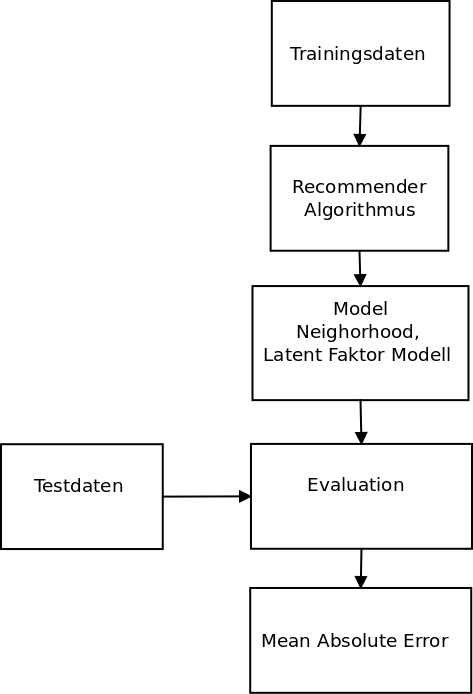
\includegraphics[width=0.5\textwidth]{evaluation}
  \caption{Kreuzvalidierung}
  \label{fig:crossvalidation}
\end{figure}

Das Model der Trainingsphase wird in der Testphase verwendet. Mit dem berechneten Model muss der Recommender zu jeder Bewertung des Testset eine Bewertung vorhersagen ohne die tats"achliche Bewertung zu kenne. Diese Vorhersage vergleicht man mit dem tats"achlichen Bewertung aus dem Testset. Die Abweichungen vom tats"achlichen Wert nennt man Residuen. 

\subsection{Evaluationsmetrik}
\label{sec:evaluationmetrik}

Die Qualit"at des Recommendersystem kann mit Evaluationsmetriken "uberpr"uft werden. Evaluationsmetriken geben Auskunft dar"uber wie gut das Recommendersystem ist. Idealerweise kann ein Recommendersystem die Bewertung f"ur einen User und ein Item vorhersagen. Statistische Genauigkeitsmetriken geben an wie weit entfernt die Vorhersage vom tats"achlichen Wert ist. 

Es gibt verschieden Evaluationsmetriken. In diesem Projekt wurde der Mean Absolute Error als Metrik verwendet. MAE vergleicht die tats"achliche Bewertung eines User f"ur ein Item mit der Bewertung, die der Recommender berechnet hat. Man bildet die Differenz von Vorhersage und tats"achlicher Bewertung. Von der Differenz wird der Betrag berechnet. Schliesslich bestimmt man die mittlere Abweichung, indem man durch Anzahl Bewertungen $N$ im Testset teilt 

Der MAE ist wie folgt definiert \cite{sarwar01}:

\begin{equation}
  \label{eq:mae}
  MAE = \frac{\sum_{i+1}^N | p_i-q_i | }{N}
\end{equation}

Je tiefer der MAE, desto besser ist die Genauigkeit des Recommender.

Root Mean Squared Error und Correlation sind zwei weitere Metriken.

\section{Unpers"onliche Empfehlungstechniken}
\label{sec:simple}

Dieser Abschnitt beschreibt einfache, alternative, M"oglichkeiten relative gute Empfehlungen zu generieren. Diese Techniken werden in den nachfolgenden Abschnitten als Baselinealgorithmus verwendet um zu "uberpr"ufen, ob das Recommendersystem eine h"ohere Genauigkeit erzielt. So ist einfach ersichtlich, ob die Collaborative Filtering Algorithmen einen qualitativen Vorteil bringen.

Um einem User Items zu empfehlen werden oft einfache Statistiken berechnet. Diese Methoden sind unpers"onlich. Das heisst die Top-N Empfehlungen sind nicht vom pers"onlichem Geschmack von $u$ abh"angig. Jeder User erh"alt die selben Empfehlungen. 

Diese Technik wird in vielen Bereichen angewendet. Restaurantf"uhrer oder Filmkritikwebseiten erstellen oft Ranglisten, welche Restaurants oder Filme von allen Usern im Durchschnitt am besten bewertet werden. Items mit den h"ochsten Durchschnittswerten, werden dem User empfohlen.

Die einfachste Methode eine unbekannte Bewertung abzusch"atzen, ist den Durschnitt aller Bewertungen zu berechnen.

\begin{equation}
  \label{eq:avg}
  b_{u,i} = \mu
\end{equation}

Diese Methode kann noch erweitert werden, indem man die durchschnittliche Abweichung aller Bewertungen von $b_u$ und die durschnittliche Abweichung $bi$ von Item $I$ ber"ucksichtigt \cite{jannach11}.

\begin{equation}
  \label{eq:bui}
  b_{u,i} = \mu + b_u + b_i
\end{equation}

wobei

\begin{equation}
  b_u = \frac{1}{|I_i|}\sum_{i \in I_u}(r_{u,i} - \mu)
\end{equation}

und 

\begin{equation}
  \label{eq:bi}
  b_i = \frac{1}{|U_i|}\sum_{u \in U_i}(r_{u,i} - b_u - \mu)
\end{equation}

Nach folgend bezeichnet $u$ den aktiven User und $i$ das Item, f"ur das man eine Vorhersage der Bewertung haben m"ochte. $b_ui$ bezeichnet die Absch"atzung f"ur die Bewertung von User $u$ f"ur Item $i$.

\begin{equation}
  \label{eq:baseline}
  b_{u,i} = \mu + b_u + b_i
\end{equation}

Listing \ref{lst:baseline} zeigt die Implemenation der Baseline Algorithmen.

\begin{lstlisting}[caption=Baseline predictor, label=lst:baseline]
import Math.Statistics
bui :: User -> Item -> Double
bui u i = mu + bu + bi
  where mu = avg allratings
        bu = computebu u
        bi = computebu i

computebu :: User -> Double
computebu u = sum ratings / nrOfratings
              where ratings = lookup u usermap
                    nrOfratings = length ratings

computebi :: Item -> Double
computebi i = sum ratings / nrOfratings
              where ratings = lookup i itemmap
                    nrOfratings = length ratings
\end{lstlisting}

$\mu$ kann einfach berechnet werden. Das Modul \verb|Math.Statistics| stellt die Funktion \verb|avg| zur Verf"ugung. \verb|allratings| gibt eine Liste aller Bewertungen zuru"ck. \verb|usermap| und \verb|itemmap| sind Maps. Die Funktion \verb|lookup| l"auft in O(logn).

In Diagramm \ref{fig:maebaselines} werden die verschiedenen, unpers"onlichen Recommender miteinander verglichen. Die Kombination aus Durchschnitt und Abweichung vom Durschnitt kann die Bewertungen der User am besten vorhersagen. Das Diagramm zeigt den Mean Absolute Error. Dieser Wert ist kurz gesagt der Durchschnitt der Abweichung der Vorhersage von tats"achlichen Wert.

\begin{figure}
  \centering
\begin{tikzpicture}
  \begin{axis}[
    xbar, xmin=0,
    width=12cm, enlarge y limits=0.5,
    symbolic y coords = {Global-AVG,Item-AVG,User-AVG,$b_{ui}$},
    xlabel={MeanAbsoluteError},
    ytick = data,
    nodes near coords, nodes near coords align={horizontal},
    ]
    \addplot coordinates {(1.044,Global-AVG) (0.930,User-AVG) (0.877,Item-AVG) (0.861,$b_{ui}$)};
  \end{axis}
\end{tikzpicture}
  
  \caption{Vergleich: unpers"onliche Empfehlungen}
  \label{fig:maebaselines}
\end{figure}


\section{Userbased collaborative filtering}

Die Technik user-based collaborative filtering ist auch als k-NN (nearest-neighbor) oder Memory-based collaborative filtering bekannt. Der GroupLens Usenet Articel Recommender verwendete als einer der ersten Recommender Systeme User-based collaborative Filtering. Ringo Musice Recommender und der Bell Core video Recommender verwenden auch user-based CF .

User-base collaborative filtering kann in zwei Schritte aufgeteilt werden. 

\begin{enumerate}
\item Nachbarschaft erstellen
\item Aufgrund der Nachbarschaft 
\end{enumerate}

User base filtering sucht nach User, die "ahnlich sind. Eine Nachbarschaft besteht aus einem Subset von $ \mathnormal{U} $ Usern $N$, die die h"ochste "Ahnlichkeit aufweisen. Um die Nachbarschaft zu erstellen wird der aktive User mit allen anderen Usern verglichen. Zu jedem Paar wird ein Wert f"ur die "Ahnlichkeit berechnet.

Bespielsweise m"ochte man die Bewertung von User Peter f"ur den Film "Titanic", den Peter noch nicht bewertet hat, vorhersagen. Man sucht nach anderen Usern die Filme "ahnlich bewerten wie Peter. Dazu analisiert man Filme die Peter und andere User bewertet haben. Um die gesuchte Sch"atzung zu erhalten eribt sich aus den gewichteten Wertungen dieser "ahnlichen User. Die Bewertung f"ur Titanic con Usern die Peter sehr "ahnlich sind haben ein gr"osseres Gewicht als die Bewertungen von Usern die Peter unahnlich sind oder sie werden gar nicht ber"ucksichtigt.

Die Technik um "ahnliche User zu finden heisst kNN (k neirest neighbors). 

\subsection{"Ahnlichkeit}

Dieser Abschnitt beschreibt, wie die "Ahnlichkeit zwischen zwei User berechnet wird. 

Es gibt mehrere M"oglichkeiten die "Ahnlichkeit zwischen zwei User zu evaluieren. F"ur die Distanz oder die "Ahnlichkeit gibt es verschiedene Metriken. 

Es ist nur m"oglich die "Ahnlichkeit zwischen 2 User zu berechnen, wenn es ein Subset der Items gibt, die beide User bewertet haben. Wenn dieses Subset leer ist, k"onnen die nachfolgenden Methoden nicht angewendet werden. Der Recommender wurde so implementiert, dass User die keine gemeinsamen Items haben als un"ahnlich bewertet werden.

Wenn es keinen User gibt, der das selbe Item bewertet hat, ist der Korrelationskoeffizient -1.
Die Pearson Similarity ber"ucksichtigt nur gemeinsam geratete Daten.
Was passiert wenn zwei User ein einziges gemeinsames Item haben und dieses gleich bewerten?

\subsubsection{Pearson Korrelation}
\label{sec:pearsoncorrelation}

Um zwei User miteinander zu vergleichen, kann die Pearson Similarity eingesetzt werden.

Wenn man zwei User mit dem Pearson Korrelationskoeffizient vergleichen m"ochte, muss man zuerst alle Items finden die beide User bewertet haben. Wenn die beiden User alle gemeinsamen Items gleich bwertet haben, sind sie sich "ahnlich.

Die Pearson Similariy ber"ucksichtig User die Items konstant tiefer bewerten. Wenn man zwei User die mit den Vektoren (1,2,3,4) und (2,3,4,5) dargestellt werden erhalten die maximale "Ahnlichkeit von 1.

\begin{equation}
 sim(u,v) = \frac{cov(X,Y}{\sigma_X \sigma_Y)} = \frac{(r_{u,i} - \bar{r}_u)(r_{v,i} - \bar{r}_v)}{r_{v,i} - \bar{r}_v}    
\end{equation}

Wenn man diese Formel auf den Vergleich von zwei Usern anwendet, kommt folgendes heraus.
\begin{equation}
 sim(u,v) = \frac{\sum_{i \in I_u \cap I_v} (r_{u,i} - \bar{r}_u)(r_{v,i} - \bar{r}_v)}{\sqrt{\sum_{i \in I_u \cap I_v}(r_{u,i} - \bar{r}_u)^2}\sqrt{\sum_{i \in I_u \cap I_v}(r_{v,i} - \bar{r}_v)^2}}
\end{equation}

Bei der verwendung der Pearson Korrelation treten mehrere Schwierigkeiten auf.

Die Berechnung Pearson Korrelation zwischen zwei Usern die nur ein Item gemeinsam bewertet haben f""uhrt zu relativ hohen "Ahnlichkeitswerten, obwohl zwei User die nur ein gemeinsames Item haben eher un"ahnlich sind.

Wenn aller gemeinsamen Items 0 ist. Das heisst wenn alle gemeinsamen Items von einem User gleich beweret wurde, der Nenner 0 und somit ist die Pearson Korrelation nicht definiert.

F"ur die Berechnung des Pearson Korrelationskoeffizienten wurde das bestehende Modul Math.Statistics eingesetzt. Listing \ref{lst:similarity} zeigt die Implementation der Similarityfunktion in Haskell.

Die Funktion \verb|pearson :: Floating a=>[a]->[a]->a| berechnet den Pearson Korrelations Koeffizienten.

\begin{lstlisting}[caption=Similarity, label=lst:similarity]
similarity :: User -> User -> Maybe Double
similarity u v = Statistics.pearson r1 r2
                 where (r1, r2) = ratings

ratings::User->User->([Double],[Double])
rarings u1 u2=(lookupR u1 shared, lookupR u2 shared)
  where shared = shareditems u1 u2

lookupR::User->[Item]->Maybe[Double]
lookupR u is = do
  ratingmap <- lookup u useritemMap
  foldl (\acc x -> (lookup x ratingmap):acc) [] is
\end{lstlisting}

Um die Similarity zwischen zwei User zu berechnen muss der \verb|pearson| Funktion die Ratings aller gemeinsamen bewerteten Items "ubergeben. In einem ersten Schritt muss eine Liste mit Items, die beide User \verb|u1| und \verb|u2| erstellt werden. Die Funktion \verb|shareditems| gibt eine Liste mit Items zur"uck die beide User bewertet haben. Listing \ref{lst:shareditems} zeigt die Implementation von \verb|shareditems|.

\begin{lstlisting}[caption=shareditems, label=lst:shareditems]
shareditems :: User -> User -> [Item]
shareditems u1 u2==[x|i1<-is1,i2<-is2,x == y]
  where is1=lookup u1 itemMap
        is2=lookup u2 itemMap
\end{lstlisting}
n
Sobald man die gemeinsam bewerteten Items hat und die dazugeh"origen Bewertungen der User kann man die Bewertungen der \verb|pearson|-Funktion "ubergeben. Diese gibt die "Ahnlichkeit der User $u$ und $v$ zur"uck. Die "Ahnlichkeit wird mit einer Gleitkommazahl zwischen -1 und 1 ausgedr"uckt. 1 bedeuted sie sind gleich. -1 bedeutet sie sind sich un"ahnlich.

\subsubsection{Euklidische Distanz}
\label{sec:euclid}

Da der Pearson Korrelations Koeffizient nicht definiert ist, wenn die Varianz 0 ist wird in diesem Fall eine alternative Distanzmetrik angewendet. Die euklidische Distanz ist auch definiert wenn die Varianz 0 ist.

Jede Wertung entspricht dem Wert einer Dimension. Die euklidische Distanz berechnet einfach den geometischen Abstand.

\begin{equation}
  \label{eq:euclid}
 sim(u,v) = \sum_i^n (u_i - p_i )^2
\end{equation}

Die euklidische Distanz ber"ucksichtigt nicht, dass bestimmte User permanent h"ohere Wertungen geben.

\subsection{Unbekannte Bewertung absch"atzen}
\label{sec:compp}

Sobald man die "Ahnlichkeiten zwischen allen Usern ausgerechnet hat, kann man f"ur einen User $u$ und ein Item $i$, eine Bewertung oder die Wahrscheinlichkeit, dass der User das Item kaufen w"urde, absch"atzen.

Die Berechnung kann in zwei Schritte aufgeteilt werden:
\begin{description}
\item[Nachbarschaft bestimmen] F"ur User $u$ wird eine Nachbarschaft $N \subseteq U$ erstellt. Diese Nachbarschaft enth"alt Tupel mit anderen Usern und deren "Ahnlichkeit zu $u$. Die Nachbarschaft ist sortiert nach "Ahnlichkeit. Die Nachbarschaft wird aufgrund der Trainingsdaten erstellt. Sie stellt das Model von user-based Collaborative Filtering dar. Wenn im zweiten Schritt eine unbekannte Bewertung abgesch"atzt werden soll wird auf die vorberechneten Nachbarschaften zugegriffen.
\item [gewichtetes Mittel bilden] Wenn man $N$ hat, nimmt man daraus $k$ "ahnliche User aus $N$, die das Item $i$ bewertet haben. F"ur alle User dieser Schnittmenge, multipliziert man das Rating des entsprechenden Users mit dem Wert der Similarity zu $u$. Dadurch werden Ratings von User, die sehr "ahnlich sind st"arker gewichtet. Man berechnet den Durchschnitt dieser Ratings. Um die gesch"atzte Bewertung zu normieren, wird die Summe der gewichteteten Bewertungen durch die Summe aller Gewichte geteilt. Gleichung \ref{eq:computeprediction} beschreibt die Berechnung von $p_{u,i}$ formel.
\end{description}

M"ochte man f"ur einen User $u$ f"ur ein bestimmtes Item $i$, das er noch nicht bewertet hat, eine Bewertung vorhersagen, kann man also folgende Formel anwenden.

\begin{equation}
  \label{eq:computeprediction}
  p_{u,i} = \frac{\sum_{u' \in N}{s(u,u') r_{u',i}}}{\sum_{u' \in N}{|s(u,u')|}}
\end{equation}

$N$ sind alle User, die das Item $i$ bewertet haben. $s$ ist eine Funktion die einen Wert f"ur die "Ahnlichkeit zwischen dem gew"unschten User $u$ und dem User $u'$ in der Nachbarschaft $N$ bestimmt.

Bei der Berechnung von $p_{u,i}$ kann die Gr"osse der Nachbarschaft $N$ frei gew"ahlt werden. Die Gr"osse der Nachbarschaft ist definiert als Parameter $k$. Wenn $k$ zu klein ist, werden nur wenige Bewertungen von anderen User zu Berechnung verwendet. Da $p_{u,i}$ in diesem Fall nur von wenigen anderen Usern abh"angig ist, ist es anf"allig f"ur Ausreisser. Wenn $k$ zu gross gew"ahlt wird, werden auch die Bewertungen der User die dem aktiven User un"ahnlich sind ber"ucksichtigt. Diese Bewertungen sind f"ur den aktiven User nicht interessant. 

Die Implementation der Gleichung \ref{eq:computeprediction} ist in Listing \ref{lst:knnpredict} dargestellt. Die Funktion \verb|predict| nimmt User, Item, Model und $k$ als Argument. Das Model enth"alt die vorberechneten Nachbarschaften. Die Funktion \verb|knn| greift darauf zu und stellt die Nachbarschaft f"ur den aktiven User und dem gew"unschten Item zusammen.

\begin{lstlisting}[caption=Berechnung von $p_{u,i}$, label=lst:knnpredict]
  predict :: User
   -> Item
   -> Model
   -> Int
   -> Double
predict user item model k = rating / normalization
  where neighborhood = knn user item model k
        normalization = sum [ s | (s,_,_) <- neighborhood]
        rating = sum [s * r | (s, r, u) <- neighborhood]
\end{lstlisting}

\subsection{Resultate}
\label{sec:userbasedresults}

In diesem Abschnitt werden die Resultate der Evaluation von Userbased Collaborative Filtering pr"asentiert. Userbased Collaborative Filtering nimmt zwei Parameter.
\begin{itemize}
\item "Ahnlichkeitsmetrik
\item Nachbarschaftsgr"osse $k$
\end{itemize}

In diesem Projekt wurden zwei A"hnlichkeitsmetriken implementiert.

\begin{itemize}
\item Euklidische Distanz
\item Pearson Correlation
\end{itemize}

F"ur jede "Ahnlichkeitmetrik wurde ein Userbased-Model mit dem Trainingset erstetllt. Diese wurden mit dem Testset evaluiert. Der Vegleich der "Ahnlichkeitmetriken wurde mit einer Nachbarschaftsgr"osse $k$ von 30 erstellt.

\begin{figure}
  \centering
\begin{tikzpicture}
  \begin{axis}[
    xbar, xmin=0.8,
    height=4.5cm, width=12cm, enlarge y limits=0.5,
    symbolic y coords = {Euklidische Distanz,Pearson Korrelation},
    xlabel={MeanAbsoluteError},
    ytick = data,
    nodes near coords, nodes near coords align={horizontal},
    ]
    \addplot coordinates {(0.872,Euklidische Distanz) (0.831,Pearson Korrelation)};
  \end{axis}
\end{tikzpicture}
\label{fig:similarity}
\caption{Vergleich der "Ahnlichkeitsmetriken euklidische Distanz und Pearson Korrelation}
\end{figure}

Der Vergleich der "Ahnlichkeitsmetriken zeigt, dass der Userbased Collaborative Filtering Algorithmus bessere Bewertungen mit dem Pearson Korrelation sch"atzt.

Die Gr"osse der Nachbarschaft $k$ hat grossen Einfluss auf die Qualit"at des Recommender. Um den besten Wert f"ur $k$ herauszufinden wurden mehrere Testl"aufe mit unterschiedlichem $k$ ausgef"uhrt.

\begin{figure}
  \centering
\begin{tikzpicture}
  \begin{axis}[
    title=Sensitiv"at der Nachbarschaftsgr"osse,
    xlabel=Anzahl Nachbarn,
    ylabel=MAE,
]
\addplot table {kdata.dat};
  \end{axis}
\end{tikzpicture}
\label{fig:nrofneighbors}
\caption{Vergleich der "Ahnlichkeitsmetriken euklidische Distanz und Pearson Korrelation}
\end{figure}

Abbildung \ref{fig:nrofneighbors} zeigt den Mean Absolute Error in Abh"angigkeit der Nachbarschaftsgr"osse $k$. F"ur das gegebene Testset funktioniert eine Nachbarschaftsgr"osse von 30 am besten.

Im Vergleich zur unpers"onlichen Bewertungsberechnung \ref{eq:bui}, generiert der User-based Collaboritive Filtering Algorithmus Bewertungen, die einen tieferen Mean Absolute Error zur Folge haben.

\begin{figure}
  \centering
\begin{tikzpicture}
  \begin{axis}[
    xbar, xmin=0.8,
    height=4.5cm, width=12cm, enlarge y limits=0.5,
    symbolic y coords = {Userbased,$b_{ui}$},
    xlabel={MeanAbsoluteError},
    ytick = data,
    nodes near coords, nodes near coords align={horizontal},
    ]
    \addplot coordinates {(0.831,Userbased) (0.861,$b_{ui}$)};
  \end{axis}
\end{tikzpicture}
\label{fig:uuvsbui}
\caption{Vergleich von Userbased CF mit unpers"onlichen Empfehlungen}
\end{figure}

F"ur den Vergleich von Abbildung \ref{fig:uuvsbui} wurde der Userbased Algorithmus mit einer Nachbarschaftsgr"osse von 30 und mit der Pearson Korrelation Metrik ausgef"uhrt. 

Wie man Abbildung \ref{fig:uuvsbui} entnehmen kann bringt Userbased Collaborative Filtering einen qualitativen Vorteil. Der Algorithmus ist intuitiv und relative einfach zu implementieren. Da er nur zwei Paramter hat ("Ahnlichkeitsmetrik, Nachbarschaftsgr"osse) kann man den Algorithmus einfach einsetzen. Wenn man gute Map Implementationen zur Verf"ugung hat, kann eine Bewertung in vern"unftiger Zeit abgesch"atzt werden.

\section{Matrix Faktorisierung}
\label{sec:matrixfactorization}

Collaborative Filtering kann man weiter noch in neighborhood methods und latent factor model aufteilen. Bei Neighborhood Methoden geht es darum "ahnliche User oder Items zu finden. Latent Factor Models versuchen die Items und die User zu charakterisieren. 

Man geht davon aus Users und Items sogenannte Latent Factors haben. Das heisst ein User hat zum Beispiel bestimmte Preferenzen. Diese Preferenzen kann mit einem Vektor repr"asentiert werden. Jedes Element sagt aus, ob dem User eine bestimmte Eigenschaft wichtig ist oder nicht. Ein User der Action mag aber keine Romanze k"onnte zum Beispiel durch folgenden Vektor repr"asentiert werden.

\begin{equation}
  \label{eq:vektor}
  p_u = \left(
  \begin{array}[c]{c}
    5 \\
    1 
  \end{array}
\right)
\end{equation}

Die 5 repr"asentiert Action und die 1 repr"asentiert die den Romantik Preferenz.

 Ein Film kann ebenfalls nach den selben Dimensionen bewertet werden. Ein Vektor kann beschreiben wie actiongeladen oder wie romantisch ein Film ist. Das Rating ist das Skalarprodukt der Preferenzen des Users und den Eigenschaften des Items.

Beim Latent Factor Ansatz ist es nicht relevant, welche Bedeutung die Elemente in den Featurevektoren haben. Es geht nur darum die Muster zu finden. Matrixfaktorierung generiert Vektoren f"ur Eigenschaften, die wir gar nicht interpretieren k"onnen.

Abbildung \ref{fig:moviedimension} veranschaulicht die Idee.

\begin{figure}
\centering
\begin{tikzpicture}[inner sep=5pt]
\begin{axis}[nodes near coords,enlargelimits=0.5]
\addplot+[only marks,
point meta=explicit symbolic]
coordinates {
(0.5,0.3) [Braveheart]
(0.2,0.1) [Oceans 11]
(0.6,0.9) [Lord of the Rings]
(0.35,0.5) [Rambo 4]
(0.6,0.1) [99 francs]
};
\end{axis}
\end{tikzpicture}
\label{fig:moviedimension}
\end{figure}

\subsection{Matrixfaktorisierung Model}
\label{sec:matrixfactorizationmodel}

Das Model der Matrixfaktorisierung weist jedem User und jedem Item einen Latent Factor Vektor der L"ange $f$ zu. Jedes Item kann durch einen Vektor $q_i \in \mathbb{R}^f$ repr"asentiert werden und jeder User kann durch einen Vektor $p_u \in \mathbb{R}^f$ repr"asentiert werden. Wenn man die Bewertung von Item $i$ f"ur User $u$ absch"atzen m"ochte, kann man das Vektorprodukt von $q_i$ und $p_u$ berechnen.

\begin{equation}
  \label{eq:rui}
  \hat(r_{ui}) = q_i^T p_u
\end{equation}

$\hat(r_{ui})$ bescheibt wie gut die Preferenzen des Users $u$ mit den Eigenschaften des Items $i$ "ubereinstimmen. Das nennt man die Interaktion zwischen User und Item.

In Haskell l"asst kann die Gleichung \ref{eq:rui} kann einfach umgesetzt werden. Das Module \verb|Data.Vector| aus dem Package \verb|vector| stellt die Funktion \verb|vdot| zur Verf"ugung. Die Implemantation ist in Listing \ref{lst:rui} dargestellt.

\begin{lstlisting}[caption=Implementation der Vorhersage, label=lst:rui]
import module Data.Vector
rui:: Vector -> Vector -> Double
rui qi pu = vdot qi pu
\end{lstlisting}

\subsection{Dimensions Reduktion}
\label{sec:dimred}

Repr"sentiert man die User-Item Interaktion mit der Ratingmatix ben"otigt man 

\begin{equation}
  \label{eq:dimre}
  1682 * 943 = 1586126
\end{equation}

Eintr"age. Diese 1,5M Eintr"ge m"ussen alle berechnet werden. Wenn man die Interaktion zwischen User und Item mit Latent Factor Vektoren mit 40 Faktoren repr"asentiert ben"otigt man 

\begin{equation}
  \label{eq:dimred}
  40(1682*943) = 105000
\end{equation}

Eintr"age. Das sind mehr als 15-mal weniger. Mit den Latent Factor Vektoren kann man die Interaktion zwischen User und Item kompakter darstellen.

\subsection{Optimierung}
\label{sec:optim}

Bei Matrixfactorization geht es darum, die Latent Factor Vektoren $q_i$ und $q_u$ f"ur jedes Item und jeden User abzusch"atzen. Sobald alle alle Latent Factor Vektoren bekannt sind ist es mit Gleichung \ref{eq:rui} einfach die Bewertung eines User f"ur ein Item abzusch"atzen.

Diese Latent Factors m"ussen aus den gegebenen Bewertungen der User abgeleitet werden. Die Bewertungen k"onnen als Item-User Matrix dargestellt werden. In dieser Matrix sind die meisten Zellen leer, da es nicht zu allen Item User Kombinationen Bewertungen gibt. Zu Beginn der Matrixfactorization Technik f"ullt man alle Elemente der Latent Factor Vektoren $q_i, p_u \in \mathbb{R}^f$ mit Zufallszahlen ab. Mit den vorhandenen Bewertungen kann man berechnen wie gut das die angenommenen Latent Factos sind. F"ur eine vorhandene Bewertung berechnet man den Fehler den man macht wie folgt:

\begin{equation}
  \label{eq:error}
  r_{ui} - q_i^T p_u
\end{equation}

$r_{ui}$ nennt man auch die Residuen. Die Summe aller Residuen soll minimiert werden.
Die Berechnung der Residuen f"uhrt man f"ur alle gegebenen Bewertungen durch und berechnet die Summme.

\begin{equation}
\label{eq:errorsum}
  \sum_{(u,i) \in \kappa} (r_{ui} - q_i^T p_u)
\end{equation}

$\kappa$ ist die Menge aller $(u,i)$-Paare f"ur eine explizite Bewertung gemacht wurde. Diese Menge wird auch Trainingset genannt.

Das Ziel von Matrixfactorization ist es Gleichung \ref{eq:errorsum} zu minimieren. 

\begin{equation}
  \label{eq:objective}
  \min_{q*,p*} \sum_{(u,i) \in \kappa} (r_{ui} - q_i^T p_u)
\end{equation}

Wenn man Gleichung \ref{eq:objective} minimiert, werden $q_i$ und $p_u$ so gew"ahlt, dass der Fehler f"ur die vorher bekannten Werte minimiert wird. Ziel des Recommender ist es aber den Fehler auch f"ur unbekannte Bewertungen m"oglichst klein zu halten und Overfitting zu vermeiden. Dieses Verhalten wird mit einem Regularisierungterm erreicht. Der Regularisierungsterm f"uhrt dazu, dass die Elemente von $q_i$ und $p_u$ nicht zu gross werden. Die Konstante $\lambda$ kontrolliert wie stark die Gleichung \ref{eq:objective} regularisiert wird \cite{koren2009}.

\begin{equation}
  \label{eq:optimization}
    r_{ui} - q_i^T p_u + \lambda (\lVert q \rVert^2 + \lVert p \lVert ^2)
\end{equation}

Damit die Elemente der Latent Factor Vectors nicht zu gross werden, werden sie reguliert.

\subsection{Kostenfunktion}
\label{sec:opt}

Aus der Gleichung \ref{eq:optimization} kann man eine sogenannte Kostenfunktion oder Objectivefunction herleiten. Die Kostenfunktion nimmt als Argumente die Latent Factor Vectoren und gibt eine reele Zahl zur"uck. Umso kleiner diese Zahl ist umso besser sind die Parameter gew"ahlt. Die Kostenfunktion sieht folgendermassen aus:

\begin{equation}
  \label{eq:costfunction}
  J(q_1, \dots , q_n, p_1, \dots, p_m) =  (r_{ui} - q_i^T p_u)^2 + \lambda (\lVert q \rVert^2 + \lVert p \lVert ^2)
\end{equation}
 
Um das Minimum zu finden kann beispielsweise das Verfahren Gradientenabstieg angewendet werden. Dazu wird die Kostenfunktion $J$ nach $q_i$ und nach $p_u$ abgeleitet. F"ur $q_i$ lautet die Ableitung:

\begin{equation}
  \label{eq:decx}
  \frac{ \partial J }{ \partial q_i } = \sum (q_i^T p_j - r) p_j + \lambda q_i
\end{equation}

Und f"ur die $p_i$ wird folgendermassen abgeleitet:

\begin{equation}
  \label{eq:dectheta}
  \frac{ \partial J }{ \partial p_i } = \sum (q_i^T p_j - r) q_j + \lambda p_i
\end{equation}

Es hat sich herausgestellt, dass das Verfahren des Gradientenabstiegs f"ur eine Ratingmatrix mit den Dimensionen 1682 x 943 nicht skaliert. Sobald man mehrere Iterationen durchf"uhrt dauert das Verfahren mehrere Stunden. Und wenn man zu wenige Iteration durchf"uhrt, werden die Paramter nicht befriedigend optimiert.

Gradient Descent muss f"ur jeden Paramter in $J$ alle m"oglichen Fehler berechnen.

\subsection{Funk's stochastischer Gradientabstieg}
\label{sec:funksvd}

Statt des einfachen Gradient Descent wurde eine Variante der Gradient Descent Methode implementiert. Die Methode wurde von Simon Funk beschrieben \cite{funk}. Die Implementation basiert auf dieser Beschreibung.

Funk's Stochastischer Gradientenabstieg iteriert durch alle User-Item Paare des Trainingsets. Mit den initialen Latent Factor Vektoren $q_i$ und $p_u$ wird f"ur jede Bewertung im Trainingset der Fehelr berechnet. Es ist einfach die Item-User Paare des Trainingsets abzufragen. Listing \ref{lst:trainingcases} zeigt die Implementation.

\begin{lstlisting}[caption=Abfrage des Trainingsets,label=lst:trainingcases]
import qualified Data.Matrix as M  
trainingcases :: M.Matrix Double -> [(Int, Int)]
trainingcases y = [(x2, x1) | x1 <- [1..(M.ncols y)], 
         x2 <- [1..(M.nrows y)],
         (M.getElem x2 x1 y) /= 0.0 ]
\end{lstlisting}

\begin{equation}
  \label{eq:error1}
  e_{ui} = r_{ui} - q_i^T p_u
\end{equation}

Wenn man diese Gleichungen partiell nach $q_i$ und $p_u$ ableitet, erh"alt man folgende Formeln

\begin{equation}
  \label{eq:devqi}
  (r_{ui} - q_i^T p_u) * p_u =  e_{ui} * p_u
\end{equation}

\begin{equation}
  \label{eq:devpu}
    (r_{ui} - q_i^T p_u) * q_i =  e_{ui} * q_i
\end{equation}

Bei der Methode des stochastischen Gradientenabstiegs passt man jede Parameter in der Richtung des Fehlers an. Die Richtungen der Fehler sind die Ableitungen aus Gleichung \ref{eq:devqi} und \ref{eq:devpu}. Die Parameter werden also wie folgt angepasst:

\begin{equation}
  \label{eq:assignpi}
 q_i \leftarrow q_i + \alpha (e_{ui} * p_u)
\end{equation}

und

\begin{equation}
  \label{eq:assignqu}
 p_u \leftarrow p_u + \alpha (e_{ui} * q_i)
\end{equation}

$\alpha$ ist eine Konstante. Sie bestimmt mit welcher schrittweite die Paramter angepasst werden. Mehrere Testl"aufe haben ergeben, dass $\alpha = 0.001$ ein geeigneter Wert ist, der mit wenigen Iterationen schnell zum Ziel f"uhrt.

Die beiden Zuweisungen \ref{eq:assignpi} und \ref{eq:assignqu} werden f"ur alle Paare im Trainingset ausgef"uhrt. Bei jeder Zuweisung wird $e_{ui}$ neu berechnet. Daraus folgt, dass die beiden Zuweisung stark voneinander abh"angig sind.

\subsubsection{Initialisierung}
\label{sec:init}

Der Algorithmus in Abschnitt \ref{sec:funksvd} geht davon aus, dass die Vektoren $q_i$ und $p_u$ bereits initialisiert sind. Dass heisst es ist n"otig, dass man eine Initialisierungstrategie f"ur die Vektoren hat. 

Eine M"oglichkeit ist die Elemente der Vektoren mit 0.1 zu initialisieren. 

Eine weitere M"oglichkeit die Featurevektoren zu initialisieren ist die leeren Zellen Ratingmatrix auszuf"ullen. M"ogliche Werte f"ur die Zellen liefern die Formeln der unpers"onliche Empfehlungstechniken aus Abschnitt \ref{sec:simple}. F"ur jede Zelle die keine Bewertung enth"alt wird 

\begin{equation}
  \label{eq:mu2}
    b_{u,i} = \mu + b_u + b_i
\end{equation}

ausrechnet.

Aus dieser vorberechneten Ratingmatrix kann man die Latent Faktor Vektoren mit einer Singul"arwertzerlegung gewinnen.

\subsubsection{Regularisierung}
\label{sec:regularization}

Der Algorithmus in Abschnitt \ref{sec:funksvd} berechnet Featurevektoren, die das Trainingsset am besten approximieren. Das ist aber nicht gew"unschte Verhalten. Man m"ochte die Featurevektoren mit dem Trainingsset berechnen und sie sp"ater auf ein unbekanntes Set anwenden. Der Algorithmus berechnet Parameter, die sich auf das Trainingsset spezialisieren. 

Um das zu vermeiden, werden die Featurevektoren regularisiert. Das heisst, dass grosse Werte in den Elementen zu einem hohen Wert der Kostenfunktion f"uhrt. Die Zuweisung wird mit Regularisierung erweitert:

\begin{equation}
  \label{eq:assign2}
  q_i \leftarrow q_i + \alpha (e_{iu} p_u + \lambda q_i)
\end{equation}

\begin{equation}
  \label{eq:assign3}
    p_u \leftarrow p_u + \alpha (e_{iu} q_iu + \lambda p_u)
\end{equation}

$\lambda$ ist eine Konstante. Sie steuert die Regularisierung.

\subsubsection{Implementation}
\label{sec:sgdimpl}

Die Berechnung der eines einzelnen Featurevektors kann in Haskell einfach implementiert werden. Listing \ref{lst:step} zeigt die Implementation. Das Modul \verb|Data.Vector| stellt den Typ \verb|Vector| zur Verf"ugung. Dieser implementiert die Operationen \verb|(Num a => a -> Vector a -> Vector a| und \verb|(+)::(Num a) => Vector a -> Vector a|.

\begin{lstlisting}[caption=Berechnung eines Featurevektors, label={lst:step}]
import Data.Vector 
newqi :: Vector Double
  -> Vector Double
  -> Double
  -> Vector Double
newqi qi pu e = qi + alpha (e * pu - (lambda * pi))
\end{lstlisting}

Da die Datenstrukturen in Haskell immutable sind, k"onnen die Latent Faktor Vektoren $q_i$ und $p_u$ beim Updateschritt nicht einfach durch die neuen Werte ausgetauscht werden. Die Datenstruktur, die die Vektoren zusammenfasst, muss bei jedem Updateschritt neu erstellt werden. Dieser Umstand hat bei den ersten Implementation zur Lauftzeit oft eine "Out of Memory Exception" ausgel"ost. Das Problem konnte behoben werden, indem Maps statt Matrizen eingeseztzt werden. Die Maps werden bei jeder Iteration neu aufgebaut. Das heisst, es werden keine Update auf die Datenstruktur ausgef"uhrt sondern nur Inserts. Diese k"onnen in O(log n) ausgef"uhrt werden und ein Teil alten Datenstruktur kann wiederverwendet werden.

\begin{lstlisting}[caption=Implementation Funk SGD, label=lst:sgd] 
train :: Features
      -> (Int,Int) 
      -> M.Matrix Double 
      -> Features
train (x, theta) (i, u) y
  = (updateRow i newqi x, updateRow u newpu theta)
  where newqi = newqi oldqi oldpu error
        newpu = newpu oldpu oldqi error
        oldqi = M.lookup i 1 x
        oldpu = M.lookup u 1 theta
        error = eui2 (rui (i,u) y) oldqi oldpu  
\end{lstlisting}

\subsection{Resultate}
\label{sec:results}

In diesem Abschnitt werden die Resultate der Evaluierung der Matrixfaktorisierungmethode pr"asentiert.

Bei der Matrixfaktorisierung gibt es mehr Paramater als bei der Userbased Methode. Folgende Paramter k"onnen frei gew"ahlt werden.

\begin{description}
\item[$\lambda$] Bestimmt wie stark die Regularisierung Overfitting vermeiden soll
\item[Anzahl Featuers] Bestimmt wieviele Elemente die Latent Faktor Vektoren haben
\item[$\alpha$] Bestimmt die Schrittweite des Gradientenabstieg.
\item[Anzahl Iterationen] Bestimmt wieviele Iterationen der Gradientenabstieg ausf"uhren soll
\end{description}

Abbildung \ref{fig:lambda} zeigt die Kreuzvalidierung f"ur den Paramter $\lambda$. Bei dieser Evaluation wurde die Anzahl Iterationen auf 20 gesetzt und $\alpha$ auf 0.001 und es wurde ein reduziertes Datenset mit 2 Features pro Latent Faktor Vektor verwendet.
Bei dem gegebenen Datenset hat der Wert von 0.01 am besten funktioniert.

\begin{figure}
  \centering
\begin{tikzpicture}
  \begin{axis}[
    title=Sensitiv"at von $\lambda$,
    xlabel=$\lambda$,
    ylabel=MAE,
]
\addplot table {lambda.data};
  \end{axis}
\end{tikzpicture}
\label{fig:lambda}
\caption{Kreuzvaliderierung von $\lambda$ mit $\alpha$ = 0.01 20 Iterationen und 2 Features}
\end{figure}

Folgende Parameter haben sich bei den Experimenten bew"ahrt.

\begin{center}
\begin{tabular}{lr}
 Parameter           &  Wert  \\
 Lambda              &  0.02  \\
 Anzahl Iterationen  &    20  \\
 Alpha               &  0.01  \\
\end{tabular}
\end{center}

Abbildung \ref{fig:compare} zeigt einen Vergleich der verschiedenen Recommender Techniken, $b_{ui}$, Userbase Collaborative Filtering und Matrixfaktorisierung.

\begin{figure}
\begin{tikzpicture}
  \begin{axis}[
    xbar, xmin=0,
    width=12cm, enlarge y limits=0.5,
    symbolic y coords = {$b_{ui}$,Userbased,Matrixfaktorisierung},
    xlabel={MeanAbsoluteError},
    ytick = data,
    nodes near coords, nodes near coords align={horizontal},
    ]
    \addplot coordinates {(0.87,$b_{ui}$) (0.84,Userbased) (0.76,Matrixfaktorisierung)};
  \end{axis}
\end{tikzpicture}
\centering
\label{fig:compare}
\caption{}
\end{figure}

Aus der Abbildung ist ersichtlich, dass der Fehler des Recommender bei Matrixfaktorisierung am geringsten ist.

\section{Implementationsdetails}
\label{sec:ram}

Dieser Abschnitt beschreibt Probleme die bei der Implementation aufgetreten sind und m"ogliche L"osungen.

F"ur den Vergleich der beiden Algorithmen Userbased Collaborative Filtering und Matrixfaktorisierung wurden zwei Module geschrieben. Um die Empfehlungen zu Evaluieren wurde ein ausf"uhrbares Programm erstellt. Das ausf"uhrbare Programm liest die Trainingsdaten und Testdaten, erstellt ein Model und berechnet den Mean Absolute Error und schreibt diese auf den Standardoutput.

\subsection{Projekstruktur}
\label{sec:structur}

F"ur dieses Projekt wurden in ein ausf"uhrbares Programm und mehrere Module aufgeteilt. Abbildung \ref{fig:structur} zeigt die Aufteilung.

\begin{figure}
  \centering
      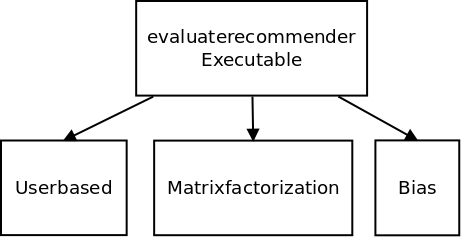
\includegraphics[width=0.5\textwidth]{structur}
  \caption{Projektstruktur}
  \label{fig:structur}
\end{figure}

\begin{description}
\item[evaluaterecommender] Diese Modul ent"halt das ausf"uhrbare Programm. Es nutzt die Module Userbased und Matrixfactorisation um die Evaluation durchzuf"uhren. Der Programmcode f"ur die MAE Berechnung ist ebenfalls in diesem Modul enthalten.
\item[Userbased] Das Modul Userbased enth"alt den User based Collaborative Filtering Recommender und die unpers"onlichen Algorithmen. Das Modul stellt die Funktion \verb|predict| und \verb|model| zur Verf"ugung
\item[Matrixfactorization] Das Modul enth"alt einen Recommender der Matrixfaktorisierung nutzt.
\item[FunkSVD] Der Optimierungalgorithmus von Simon Funk ist in diesem Modul implementiert.
\end{description}
.
atrixfactorization enth"alt einen Recommender mit Matrixfaktorisierung. Der Optimierungsalgorithmus Funk's stochatischer Gradientenabstiegt wurde in ein separates 

\subsection{Build System}
\label{sec:cabal}

Um das Projekt zu builden und die Abh"angikeiten aufzul"osen wurde Cabal eingesesetzt. Die verwendete Version ist 1.20.0.2. Cabal ein Paketisierung und Build System f"ur Haskell. In diesem Projekt wurde Cabal eingesetzt, weil Libraries des Package Repository Hackage eingesetzt wurden und Cabal kann Abh"angigkeiten zu Hackages Packages automatisch aufl"osen. Ausserdm verwaltet Cabal Projektmetadaten, wie Lizenz, Author, u.s.w.

\subsubsection{Sandboxing}
\label{sec:sanboxing}

Das Projekt wurde in einer sogenannten Sandbox erstellt. Wenn das Projekt in einer Sandbox erstellt wird, werden alle Abh"angigkeiten des Projekt in einer separaten Paketverwaltung installiert. Das hat den Vorteil, dass "Anderungen an der system globalen Paketverwaltung das Projekt nicht beinflussen. Der Befehl lautet:
\begin{verbatim}
cabal sandbox init
\end{verbatim}

\subsection{Daten einlesen}
\label{sec:readio}

Beim einlesen der Daten sollte mit \verb|ByteString| gearbeitet werden. Dieser Abschnitt beschreibt weshalb.

Bei der Ausf"uhrung der Evaluation werden die Daten jedesmal vom Filesystem eingelesen. Das Modul Pelude bietet daf"ur die Funktion \verb|readFile:: FilePath -> IO String|. \verb|FilePath| ist ein Alias f"ur \verb|String|. Die Funktion nimmt einen Dateipfad und gibt eine IO Action zur"uck. Die IO Action liest den Inhalt des Files und bindet Resultat an einen String.

Ein \verb|String| ist eine Liste. Listen werden Haskell lazy evaluiert. Ein File ist f"ur Haskell also nur eine Liste von Character. Wenn die Listen lazy evaluiert werden sind die Elemente darin nur ein Promise, dass das Element zur Verf"ugung steht, wenn es ben"otigt wird. Die Berechnung des Elements hat noch nicht stattgefunden. Das ist normalerweise kein Problem aber wenn diese Liste ein Stream von der Festplatte ist, ist das Einlesen vergleichweise langsam.

Deshalb gibt es im Paket \verb|bytestring| die Datentypen \verb|Data.ByteString.Strict| und \verb|Data.ByteString.Lazy|. Die Strict-Version l"ost das Problem indem die ganze String in den Arbeitsspeicher eingelesen wird. \verb|Data.ByteString.Lazy| liest die ersten 64KB in den Arbeitsspeicher.

Da die Trainings und Testdaten ca. 1.7MB gross sind, wurde f"ur dieses Project \verb|Data.ByteString.Strict| verwendet.

Listing \ref{lst:readio} zeigt wie Daten mit einem ByteString eingelesen werden. Der ByteString wird danach der Funktion \verb|decode| "ubergeben. Das diese ein \verb|Either| wird ein m"oglicher Fehler in der Funktion \verb|toVec| abgefangen.

\begin{lstlisting}[label={lst:readio},caption={Einlesen von Files mit ByteString}]
import Data.Csv
import qualified Data.Vector as V
import qualified Data.ByteString.Lazy as Bl

type Rating = (Int, Int, Double)

basefile = "/home/lukas/oschena/ml-100k/base.csv"

main = do
  putStrLn "Loading Data"
  c <- Bl.readFile basefile
  let csvData = decode NoHeader c :: Either String (V.Vector Rating)
  let v = toVec csvData
  putStrLn $ "Number of Ratings: " ++ (show $ V.length v)

toVec :: Either String (V.Vector Rating)
      -> V.Vector Rating
toVec (Left err) = error err
toVec (Right v) = v
\end{lstlisting}

\subsection{Profiling}
\label{sec:profiling}

Bei den ersten Implementation der Collaborative Filtering Algorithmen ist es oft zu "Memory out of Bound" Exceptions gekommen oder das Programm ben"otigte zu viel Zeit. Um Probleme der Skalierbarkeit zu l"osen wurden Statistiken "uber das Verhalten der Algorithmen zur Laufzeit erstellt.

Der GHC Compiler unterst"utzt Time und Memory Profiling. Der generierte Output zeigt, wieviel Zeit und Speicher eine Funktion verursacht. Das heisst jede Funktion hat ein sogennantes Kostencenter. Jedesmal, wenn die Funktion aufgerufen wird, werden Zeit und Memory zu den vorhandenen Werten im Kostencenter hinzugez"ahlt. Um die Werte in Kostencenter zu berechnen, generiert der Compiler zus"atlichen Code, der die Berechnung ausf"uhrt. Die zu analisierenden Programme m"ussen also mit der entsprechenden Compiler Option ausgef"uhrt werden.

Es k"onnen nur Ausf"uhrbare Dateien analisiert werden. In diesem Projekt wurde das Programm \verb|evaluaterecommender| analisiert.

Um das Profiling einzuschalten, m"ussen drei Compiler Optionen gesetzt werden. Die Optionen k"onnen im Cabalfile im ghc-options Property gesetzt werden.
\begin{verbatim}
executable evaluaterecommender
  ghc-options:	-prof -fprof-auto -rtsopts
\end{verbatim}
\begin{description}
\item[-prof] Profiling wird eingeschaltet
\item[-fprof-auto] Alle Funktionen sind Kostencenter
\item[-rtsopts] Erm"oglicht der Runtime Optionen mitzugeben
\end{description}

Alle verwendeten Pakete m"ussen mit der \verb|--enable-library-profiling|- Option kompiliert werden.

Um das Programm zu Analisieren muss es mit der Runtime Option \verb|-p| bei Ausf"uhrung mitgegeben werden. Runtime Optionen k"onnen nach dem Progamm zwischen \verb|+RTS| und \verb|-RTS| mitgegeben werden.  

\begin{verbatim}
$ evaluaterecommender +RTS -p -RTS
\end{verbatim}

Das Programm generiert eine Textdatei \verb|evaluaterecommender.prof|. Diese teilt die Analyse in drei Teile auf.

Im obersten wird beschrieben, wie lange die Ausf"uhrung gedauert hat und wieviel Speicher konsumiert wurde. Im zweiten Teil werden die Funktionen die am meisten Zeit und Speicher ben"otigen mit dem Prozentualen Anteil ausgelistet. Im letzen Teil wird das Aufrufabfolge der Funktionen in Form eines Baumes beschrieben.

\begin{verbatim}
	Wed Dec 24 15:05 2014 Time and Allocation Profiling Report  (Final)

	evaluaterecommender +RTS -p -K100M -RTS

	total time  =        0.74 secs   (741 ticks @ 1000 us, 1 processor)
	total alloc = 1,259,391,232 bytes  (excludes profiling overheads)

COST CENTRE   MODULE  %time %alloc

error            Main     34.7   52.3
updateRow2    Main     27.1   22.1
trainingcases Main      7.8    0.6
iter          Main      5.8    7.7
predict       Main      3.6    4.2

\end{verbatim}

\subsection{Arbeitsspeicher}
\label{sec:memory}



Bei einer Ratingmatrix r mit der Dimension von 1682 mal 943 konsumiert das Programm zu viel Arbeitsspeicher. Es werden 10GB angefordert. Profiling hat gezeigt die Fehler Berechnung viel Arbeitsspeicher konsumiert.

\begin{equation}
  \label{eq:squareerror}
  \sum_{(u,i) \in \kappa} (r_{ui} - q_i^T p_u)^2
\end{equation}

$\kappa$ ist die Menge aller User-Item Paare, f"ur die ein Rating bekannt ist.

\section{Fazit und Ausblick}
\label{sec:fazit}

Die Technik Matrixfakorisierung liefert genauere Vorhersagen als Userbase Collaborativ Filtering. Im Gegensatz zu Userbase Collaborative Filtering ist das Verfahren schwieriger zu implementieren und zu handhaben. Bei Matrixfaktorisierung mit Gradientenabstieg m"ussen 4 Parameter von Hand optimiert werden.

Die Implementierung von Funk's Gradientenabstiegverfahren hat sich als schwierig erwiesen. Da bei diesem Verfahren die Parametervektoren oft aktualisiert werden wird viel Speicher alloziert und der Garbage Collector muss andauernd aufr"aumen. Deshalb ist es sinnvoll zu pr"ufen, ob das Optimierungsverfahren Funks stochastischer Gradientenabstieg nicht durch ein Verfahren ersetzt werden kann, dass einfacher zu parallelisieren ist. Das Verfahren Alternating Root Squares w"urde sich hierf"ur anieten.

Mit Programmiersprache Haskell k"onnen die Recommender mit wenigen Zeilen Code implementiert werden. Das Package Repository Hackage bietet unter anderem Libraries f"ur den Umgang mit Matrizen und Vectoren. Es enth"alt auch Statistikpakete, die f"ur die Implementierung von Recommenender Systemen genutzt werden k"onnen.

Da die verwendeten Datenstrukturen Immutable sind und die meisten Funktionen keinen Seiteneffekt haben, w"urde sich die Parallelisierung der Algorithmen anbieten.

\bibliographystyle{plain}
\bibliography{a}
\end{document}